% !TEX root = ../main.tex

%% 实验记录	
%\begin{table}
%	\renewcommand\arraystretch{1.7}
%	\centering
%	\begin{tabularx}{\textwidth}{|X|X|X|X|}
%		\hline
%		Major： & Physics & Grade： & 2022 \\
%		\hline
%		Name： & 杨舒云 \& 戴鹏辉 & Student number： & 22344020 \& 22344016\\
%		\hline
%		Room temperature： & \degree C & Experimental location： &  \\
%		\hline
%		Student Signature：& \textbf{In Attachment} & Score： &\\
%		\hline
%		Experiment time：& 2024// & Teacher's Signature：&\\
%		\hline
%	\end{tabularx}
%\end{table}
\section{APL1-1-A 电阻热噪声及玻尔兹曼常量测量 \\ Experimental Record}


%---------------------------------------------------------------------
% 实验过程记录
\subsection{Content, Procedures \& Results}

% 操作步骤
\subsubsection{Operations}
本小节展示实验方案中的具体\textbf{操作步骤}。

首先，本预习报告不考虑远程测量的相关内容。现场测量实验方案如下所示：
\begin{enumerate}
	\item 实验前的梳理与排查。
	
	\item 按讲义回顾并完成“实验1.6 滤波器带宽对输出信号响应的影响”。
	
	\item 选择电阻（测量样品盒）：
	\begin{enumerate}
		\item 准备工作
		
		根据$\overline {V_n^2} = 4 k_\text{B} T R \, \Delta f$，我们应当希望测得较大的热噪声，但是考虑到低温测量有助于减少其他噪声源的影响、提高数据的准确性、验证热噪声的线性关系以及控制温漂效应；提供了更为精准的噪声数据，进而更准确地测量玻尔兹曼常数。所以我们需要仅可能的保持低温测量，这就需要考虑较大的电阻。
		
		由于缺乏实践（实际上可参考\cite{c}），\textbf{所以我们大胆考虑选择（144kΩ 或 ）98kΩ 的电阻，选择 100K到300K（室温）作为测量温度点}，参考98kΩ和100K下，噪声约为$23.25\text{nV}/\sqrt{\text{Hz}}$。
		
		进行测量时可参考：样品盒采用 3 个 1/8W 的阻值为 $R$ 的色环电阻，以“三角”对称连接方式解决因锁相放大器输入电阻所带来的输入带宽变窄的问题，其等效电阻为 $2/3R$。
		
		\item 控温与温度测量
		
		低温测量时，将样品盒插入盛有液氮的容器内，通过\textbf{调节插入深度}来调节电阻段的温度，并通过 MS6514 测温仪测量热电偶（T 型）的读数。
		
		\item 测量电阻值，预期数据按\cref{tab:TR}记录。
		
		这里需要弄清的问题是：仪器表（或者仪器上标注的数值）是否考虑了2/3的修正。但由于要用万用表实际测量，所以这个问题不太重要。
		
		另一个问题是基于误差要求，我们选取何种测量方案，最基本的当然是直接用万用表测量，需要考虑的是采样伏安法等其它方法精度是否会更高，这个建议到时候咨询老师。
	\end{enumerate} 
	
	\item 线路连接
	
	为尽量抑制环境噪声的影响，\textbf{测量选用差分（A-B）输入，电缆 BNC 接头分别连接在锁相放大器的 A 和 B 端}。
	
	\begin{figure}[h!]
		\centering
		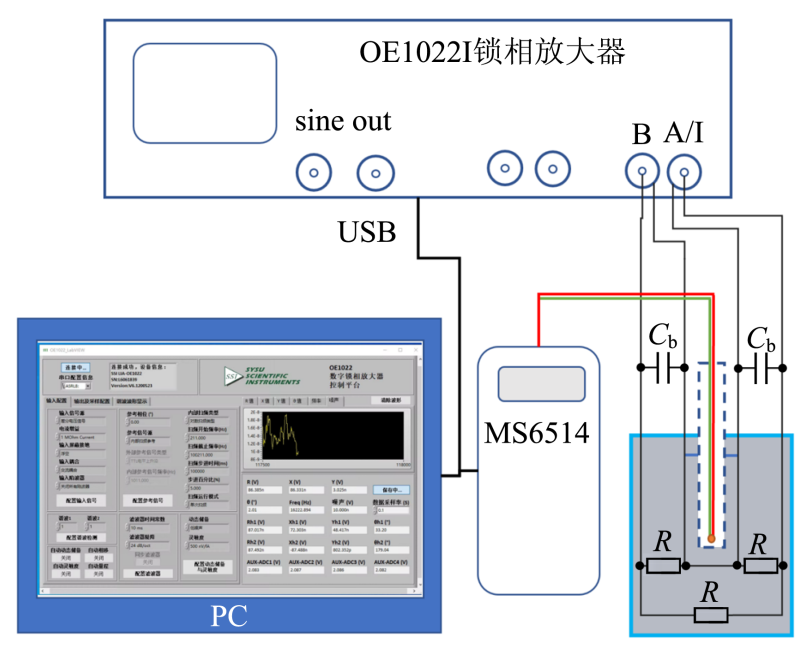
\includegraphics[width=0.5\linewidth]{images/APL1_1_A_connecting}
		\caption{电阻热噪声测量差分接线示意图（来自\cite{c}）}
		\label{fig:apl11aconnecting}
	\end{figure}
	
	仪器校正方面，此步骤中我们主要考虑\textbf{零点校正}。
	
	\item 选择仪器参数
	
	仪器的参数选择也主要参考实验讲义：
	
	\textbf{满量程灵敏度应选为 1$\mu$V；另一方面，热噪声幅值小，动态储备应选“Low Noise”。}
	
	由于测量装置不可能完全屏蔽环境干扰，选择太大的带宽容易引入近频的环境噪声，因此建议 Slope > 12dB/oct。
	
	为保证所采集的每个数据是独立的并且不失真，应该选择合适的采样的时间间隔。例如：当选时间常数 $\tau$ 为 30ms、Slope 为 18 dB/oct 时，ENBW 为 3/32 Hz，X 值的测量等待时间或时间间隔约为 $8.4\tau$（即 $\sim$250ms，见\cref{tab:ENBW}），X，Y 值同时采样 $10^3$ 个需要时间约为 4.5 分钟。
	
	由于缺乏具体实践经验，我们结合\cite{c}大胆给出\textbf{一组可能的参数选取：98kΩ 电阻，在6666Hz下，$\tau=1s$，$\text{Slope}=24\text{dB/oct}$，时间间隔$10\tau$。}
	
	\item 进行测量
	
	这个步骤中我们需要考虑\textbf{本底校正}。本底测量用 50Ω 短接，其余测量方式与所测热噪声的测量方式是相同的，注意如前文所述，本底校正一定是在选好参数后做的，换一组参数就要重做一次。预期数据记录按\cref{tab:nB}给出。
	
	接下来是正经的测量步骤，同样主要参考实验讲义。将上位 PC 机与锁相放大器相连，利用 OE1022 专用的 LabVIEW上位机采集程序对锁相放大器测量结果进行采样，采集当前锁相放大器测到的 X 值和 Y 值。采样间隔和保存路径在界面右上角 “sample” 选项卡中设置；锁相放大器参数在界面上方原理图内相关图标下的菜单中设置（这个示意图请看实验讲义）。
	
	总之，接线前和测量后请用万用表测量样品电阻， 以确认所在温度下其电阻值与标记的一致，并用于数据处理。在实验室先将线路接好； 分别打开所用锁相放大器的 LabVIEW 测量界面， 以及 MS6514 测温仪测量界面， 确认都可正常测量。 选择合适的仪器参数。 注意热电偶选“T 型” 。通过调节样品盒离液氮液面距离， 使样品自然稳定到某温度。
	
	\textbf{计划首先按前面给出的参数测量一组，后续考虑调整参数（改变频率、温度梯度等）后再测几组。}
	
	预期数据记录按\cref{tab:data1}给出。\textbf{注意实验过程拍照，测控界面截图。}
	
\end{enumerate}	

% 实验结果
\subsubsection{Display}
本小节展示预期所需的实验数据，并展示预制作的\textbf{实验数据记录表}。

\begin{table}[h!]
	\centering
	\caption{温度、电阻值数据记录表（Recorder \& Time：\hspace{4cm}）}
	\label{tab:TR}
		\begin{tabular}{|c|c|c|}
			\hline
			序号 & 温度 (K) & 电阻 (Ω) \\
			\hline
			\hspace{5cm} & \hspace{5cm} & \hspace{5cm} \\ 
			\hline
			 \hspace{5cm} & \hspace{5cm} & \hspace{5cm} \\ 
			\hline
			\hspace{5cm} & \hspace{5cm} & \hspace{5cm} \\ 
			\hline
			\hspace{5cm} & \hspace{5cm} & \hspace{5cm} \\ 
			\hline
			\hspace{5cm} & \hspace{5cm} & \hspace{5cm} \\ 
			\hline
			\hspace{5cm} & \hspace{5cm} & \hspace{5cm} \\ 
			\hline
			\hspace{5cm} & \hspace{5cm} & \hspace{5cm} \\ 
			\hline
			\hspace{5cm} & \hspace{5cm} & \hspace{5cm} \\ 
			\hline
			\hspace{5cm} & \hspace{5cm} & \hspace{5cm} \\ 
			\hline
			\hspace{5cm} & \hspace{5cm} & \hspace{5cm} \\ 
			\hline
			\hspace{5cm} & \hspace{5cm} & \hspace{5cm} \\ 
			\hline
		\end{tabular}
\end{table}

\begin{table}[h!]
	\centering
	\caption{本底测量结果记录表（Recorder \& Time：\hspace{4cm}）}
	\label{tab:nB}
	\begin{tabular}{|c|c|c|c|c|}
		\hline
		\textbf{频率 (Hz)} & \textbf{时间常数 (s)} & \textbf{陡降 (dB/oct)} & \textbf{数据存储文件名} & \textbf{备注} \\
		\hline
		\hspace{2.5cm} & \hspace{2.5cm} & \hspace{2.5cm} & \hspace{4cm} & \hspace{4cm} \\
		\hline
		\hspace{2.5cm} & \hspace{2.5cm} & \hspace{2.5cm} & \hspace{4cm} & \hspace{4cm} \\
		\hline
		\hspace{2.5cm} & \hspace{2.5cm} & \hspace{2.5cm} & \hspace{4cm} & \hspace{4cm} \\
		\hline
		\hspace{2.5cm} & \hspace{2.5cm} & \hspace{2.5cm} & \hspace{4cm} & \hspace{4cm} \\
		\hline
		\hspace{2.5cm} & \hspace{2.5cm} & \hspace{2.5cm} & \hspace{4cm} & \hspace{4cm} \\
		\hline
		\hspace{2.5cm} & \hspace{2.5cm} & \hspace{2.5cm} & \hspace{4cm} & \hspace{4cm} \\
		\hline
		\hspace{2.5cm} & \hspace{2.5cm} & \hspace{2.5cm} & \hspace{4cm} & \hspace{4cm} \\
		\hline
		\hspace{2.5cm} & \hspace{2.5cm} & \hspace{2.5cm} & \hspace{4cm} & \hspace{4cm} \\
		\hline
		\hspace{2.5cm} & \hspace{2.5cm} & \hspace{2.5cm} & \hspace{4cm} & \hspace{4cm} \\
		\hline
		\hspace{2.5cm} & \hspace{2.5cm} & \hspace{2.5cm} & \hspace{4cm} & \hspace{4cm} \\
		\hline
		\hspace{2.5cm} & \hspace{2.5cm} & \hspace{2.5cm} & \hspace{4cm} & \hspace{4cm} \\
		\hline
	\end{tabular}
\end{table}

\begin{table}[h!]
	\centering
	\caption{实验参数预置值（Recorder \& Time：\hspace{4cm}）}
	\label{tab:data1}
	\begin{tabular}{|p{4cm}|p{4cm}|p{4cm}|}
		\hline
		\textbf{输入方式} &  & \\ \hline
		\textbf{量程灵敏度} &  & \\ \hline
		\textbf{动态储备} &  & \\ \hline
		\textbf{时间常数（s）, >0.01} & & \\ \hline
		\textbf{陡降（dB/oct），$\neq$ 6} & & \\ \hline
		\textbf{远程/现场} & & \\ \hline
		\textbf{温度 1/电阻值 1} & & \\ \hline
		\textbf{温度 2/电阻值 2} & & \\ \hline
		\textbf{采样时间间隔（s）} & & \\ \hline
		\textbf{采样等待时间（s）} & & \\ \hline
		\textbf{单频点采样时长（s）} & & \\ \hline
		\textbf{单频点样本量} &  & \\ \hline
		\textbf{频率（kHz）} & & \\ \hline
		\textbf{文件名} & & \\ \hline
	\end{tabular}
\end{table}

\begin{table}[h!]
	\centering
	\caption{实验参数预置值（Recorder \& Time：\hspace{4cm}）}
	\label{tab:data2}
	\begin{tabular}{|p{4cm}|p{4cm}|p{4cm}|}
		\hline
		\textbf{输入方式} &  & \\ \hline
		\textbf{量程灵敏度} &  & \\ \hline
		\textbf{动态储备} &  & \\ \hline
		\textbf{时间常数（s）, >0.01} & & \\ \hline
		\textbf{陡降（dB/oct），$\neq$ 6} & & \\ \hline
		\textbf{远程/现场} & & \\ \hline
		\textbf{温度 1/电阻值 1} & & \\ \hline
		\textbf{温度 2/电阻值 2} & & \\ \hline
		\textbf{采样时间间隔（s）} & & \\ \hline
		\textbf{采样等待时间（s）} & & \\ \hline
		\textbf{单频点采样时长（s）} & & \\ \hline
		\textbf{单频点样本量} & & \\ \hline
		\textbf{频率（kHz）} & & \\ \hline
		\textbf{文件名} & & \\ \hline
	\end{tabular}
\end{table}

\begin{table}[h!]
	\centering
	\caption{实验参数预置值（Recorder \& Time：\hspace{4cm}）}
	\label{tab:data3}
	\begin{tabular}{|p{4cm}|p{4cm}|p{4cm}|}
		\hline
		\textbf{输入方式} &  & \\ \hline
		\textbf{量程灵敏度} &  & \\ \hline
		\textbf{动态储备} &  & \\ \hline
		\textbf{时间常数（s）, >0.01} & & \\ \hline
		\textbf{陡降（dB/oct），$\neq$ 6} & & \\ \hline
		\textbf{远程/现场} & & \\ \hline
		\textbf{温度 1/电阻值 1} & & \\ \hline
		\textbf{温度 2/电阻值 2} & & \\ \hline
		\textbf{采样时间间隔（s）} & & \\ \hline
		\textbf{采样等待时间（s）} & & \\ \hline
		\textbf{单频点采样时长（s）} & & \\ \hline
		\textbf{单频点样本量} &  & \\ \hline
		\textbf{频率（kHz）} & & \\ \hline
		\textbf{文件名} & & \\ \hline
	\end{tabular}
\end{table}

\begin{table}[h!]
	\centering
	\caption{实验参数预置值（Recorder \& Time：\hspace{4cm}）}
	\label{tab:data4}
	\begin{tabular}{|p{4cm}|p{4cm}|p{4cm}|}
		\hline
		\textbf{输入方式} &  & \\ \hline
		\textbf{量程灵敏度} &  & \\ \hline
		\textbf{动态储备} &  & \\ \hline
		\textbf{时间常数（s）, >0.01} & & \\ \hline
		\textbf{陡降（dB/oct），$\neq$ 6} & & \\ \hline
		\textbf{远程/现场} & & \\ \hline
		\textbf{温度 1/电阻值 1} & & \\ \hline
		\textbf{温度 2/电阻值 2} & & \\ \hline
		\textbf{采样时间间隔（s）} & & \\ \hline
		\textbf{采样等待时间（s）} & & \\ \hline
		\textbf{单频点采样时长（s）} & & \\ \hline
		\textbf{单频点样本量} &  & \\ \hline
		\textbf{频率（kHz）} & & \\ \hline
		\textbf{文件名} & & \\ \hline
	\end{tabular}
\end{table}

%---------------------------------------------------------------------
%% 原始数据
%\subsection{Original Data}
%The original data in the experimental notebook is shown in %\cref{} (signed).
%
%See the \textbf{Attachment} section for the clean of the experimental bench desktop (%\cref{}).
%
%Other raw data are shown in %\cref{}.


%---------------------------------------------------------------------
%% 问题记录
%\subsection{Difficulties}
%\begin{enumerate}
%	\item 
%\end{enumerate}